\documentclass[aps,prd,twocolumn,superscriptaddress,floatfix,nofootinbib]{revtex4-2}
\usepackage{amsmath,amssymb,bm,graphicx,booktabs}
\usepackage[colorlinks=true,linkcolor=blue,citecolor=blue,urlcolor=blue]{hyperref}

\begin{document}

\title{Critical coupling of compact U(1) lattice gauge theory\\ on the four-dimensional $D_4$ lattice}

\author{M.~R.~Cabri\'e}
\affiliation{Independent researcher, Victoria, Australia}

\date{DRAFT v0.1, 23 November 2026 --- not yet submitted}

\begin{abstract}
We measure the confinement--Coulomb transition of pure compact U(1) gauge theory with the
Wilson action on the $D_4$ root lattice (the vertex set of the 16-cell honeycomb), where the
elementary loops are triangles. Two independently written Monte Carlo codes, the second run
blind to the first, place the transition of the $L=8$ lattice in the same interval,
$0.610<\beta<0.615$. Mixed-phase starts at $L=12$ and $L=16$ give
$\beta_c = 0.6150(13)$ for the coefficient of the sum over triangles, equivalent to
$1/e^2_c = 2\beta_c = 1.2300(25)$ in continuum normalisation. This is $21.7\%$ above the
hypercubic value $1.0111$, so the critical bare coupling is not universal across
four-dimensional lattices even when normalised to the same continuum action. The energy jump
and the absence of tunnelling are those of a discontinuous transition, but we do not claim a
determination of the order. Both codes are calibrated on the hypercubic lattice. All code and
raw time series are public.
\end{abstract}

\maketitle

\section{Introduction}

Compact U(1) gauge theory in four dimensions has a confining phase at strong coupling and a
Coulomb phase with a massless photon at weak coupling~\cite{Wilson1974,BMK1977,Guth1980,FS1982}.
On the hypercubic lattice with the Wilson action the two are separated by a transition at
$\beta_c \simeq 1.011$ whose order was debated for two decades and is now established as weakly
first order~\cite{JNZ1983,Arnold2003}.

Almost everything known numerically about this transition has been obtained on the hypercubic
lattice. The $D_4$ lattice, the densest lattice packing in four dimensions, has 24 nearest
neighbours per site, a symmetry group of order 1152 instead of 384, and triangles instead of
squares as its smallest closed loops. Celmaster introduced it for SU($N$) gauge theory in the
1980s~\cite{Celmaster1982}, and Katz and Nogradi have recently studied SU(3) and quenched QCD
on it~\cite{KatzNogradi2026}. We are not aware of any published result for U(1) on this lattice,
or on any non-hypercubic four-dimensional lattice.

The question addressed here is narrow: where is the transition on $D_4$, and is the critical
coupling the same as on the hypercubic lattice once both are expressed through the same
continuum action? It is not. We make no claim about a continuum limit; the transition is a
lattice phenomenon, and on the hypercubic lattice it is first order.

\section{Lattice and action}

Sites are the points of $\mathbb{Z}^4$ with even coordinate sum, in a periodic box of side $L$
($L^4/2$ sites). Each site has 24 nearest neighbours at $(\pm1,\pm1,0,0)$ and permutations, so
there are 12 links per site. Three mutually nearest sites form an equilateral triangle; there
are 32 triangles per site and 8 through every link. The link variables are phases
$\theta_\ell\in(-\pi,\pi]$, and
\begin{equation}
S=\beta\sum_{\triangle}\bigl(1-\cos\theta_\triangle\bigr),
\label{eq:action}
\end{equation}
where $\theta_\triangle$ is the oriented sum of the three link phases around a triangle.

Expanding Eq.~\eqref{eq:action} for smooth fields and summing the squared area bivectors of
the 32 triangles gives $S\to\frac{1}{4e^2}\int d^4x\,F_{\mu\nu}F_{\mu\nu}$ with
\begin{equation}
\frac{1}{e^2}=2\beta .
\end{equation}
The same expansion on the hypercubic lattice gives $1/e^2=\beta$. The normalisation of
Ref.~\cite{KatzNogradi2026} corresponds to $\beta_{\rm KN}=2\beta$. We have checked the
factor 2 by direct summation over the 32 triangles for random field strengths.

\section{Method}

Two codes were written from the same specification of lattice and action and nothing else.
Code~A updates all links of one direction at once with a vectorised heat bath on a lattice
stored as two parity copies. Code~B uses a sequential single-link heat bath, drawing each link
exactly from its conditional von Mises distribution~\cite{BestFisher1979}, on a single parity
copy, with a different random number generator. One sweep is one update of every link. Code~B
was written and run without access to the results of code~A; its numbers were hashed before
the comparison was made. The protocol of each run, including grids, sweep counts and decision
rules, was fixed in a public pre-registration before the run.

The observable is the mean triangle energy $E=\langle 1-\cos\theta_\triangle\rangle$ and its
fluctuation $C=N_\triangle\,{\rm var}(E)$.

\emph{Checks (code~B).} Gauge invariance holds to $4\times10^{-15}$. At $\beta=0.1$,
$\langle\cos\theta_\triangle\rangle=0.05027(10)$, against $u+3u^3=0.05031$ from the
strong-coupling series with $u=I_1(\beta)/I_0(\beta)$; the cubic term arises because each
triangle is a face of three tetrahedra. At $\beta=20$, $E=0.008612(4)$ against the
leading weak-coupling value $11/(64\beta)=0.008594$.

\emph{Calibration.} On the hypercubic lattice at $L=8$ code~B finds the maximum of $C$ at
$\beta=1.0075$, the known pseudo-critical value for that size, and mixed-phase starts at
$L=12$ flip between $\beta=1.007$ and $1.012$, which contains the infinite-volume value
$1.0111$~\cite{Arnold2003}.

\emph{Mixed-phase starts.} Near a discontinuous transition thermal scans on large lattices
stay in the phase they start in. We therefore start from a configuration that is ordered
($\theta=0$) in one half of the box and random in the other~\cite{Creutz1979}, run 2000 sweeps, and
record which phase takes over, judged by the mean of $E$ over the last 500 sweeps against a
band of half-width $0.01$ centred on the midpoint $E^*=0.4548$ of the two branches. $\beta_{\rm mix}(L)$ is the
midpoint of the interval in which the outcome flips.

\section{Results}

\begin{figure}[b]
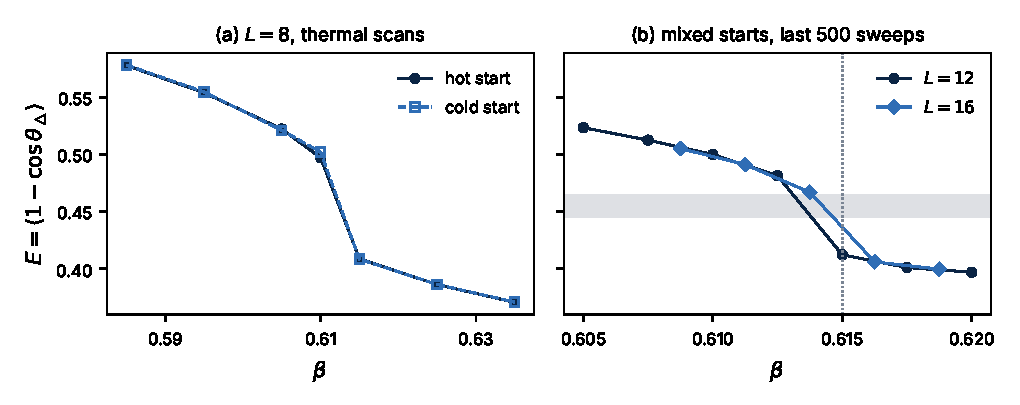
\includegraphics[width=\columnwidth]{fig1.pdf}
\caption{Code~B on $D_4$. (a) Thermal scans at $L=8$ from hot and cold starts
(2000 thermalisation and 4000 measurement sweeps). (b) Mixed-phase starts at $L=12$ and
$L=16$: mean energy over the last 500 of 2000 sweeps. The grey band separates the two
outcomes; the dotted line marks $\beta_c$.}
\label{fig:one}
\end{figure}

\begin{table}[b]
\caption{Location of the transition on $D_4$. Intervals are the adjacent grid points between
which the phase changes.}
\label{tab:one}
\begin{ruledtabular}
\begin{tabular}{llll}
code & $L$ & method & interval in $\beta$ \\
\hline
A & 8  & scan, hot and cold & $[0.610,\,0.615]$ \\
B & 8  & scan, hot and cold & $[0.610,\,0.615]$ \\
B & 12 & scan, cold         & $[0.610,\,0.615]$ \\
B & 12 & mixed start        & $[0.6125,\,0.6150]$ \\
B & 16 & mixed start        & $[0.61375,\,0.61625]$ \\
\end{tabular}
\end{ruledtabular}
\end{table}

Table~\ref{tab:one} and Fig.~\ref{fig:one} summarise the runs. At $L=8$ both codes, from both
starts, find the strong-coupling phase at $\beta=0.610$ ($E\simeq0.50$) and the weak-coupling
phase at $0.615$ ($E\simeq0.41$), a fall of $0.09$ in one grid step of $0.005$. No run
tunnelled between phases in 4000 sweeps.

The mixed starts give $\beta_{\rm mix}(12)=0.61375$ and $\beta_{\rm mix}(16)=0.6150$. Every
run resolved to one phase, the outcomes are monotonic in $\beta$, and no grid extension was
needed. We quote
\begin{equation}
\beta_c=0.6150(13),\qquad \frac{1}{e_c^2}=2\beta_c=1.2300(25),
\label{eq:result}
\end{equation}
where the value is $\beta_{\rm mix}(16)$ and the uncertainty is the larger of half the $L=16$
flip interval and the shift from $L=12$ to $L=16$, which happen to be equal. The uncertainty
is a bracketing width, not a statistical standard error: each grid point is a single run.

In continuum normalisation the ratio to the hypercubic value is
\begin{equation}
\frac{(1/e_c^2)_{D_4}}{(1/e_c^2)_{\rm hc}}=\frac{1.2300(25)}{1.0111}=1.217(3).
\end{equation}

\emph{Order of the transition.} Three observations point to a discontinuous transition:
the jump of $0.09$ in $E$ at $L=8$ and $L=12$ within one grid step; the absence of tunnelling
at any size; and the fact that a two-phase starting configuration is driven wholly into one phase or
the other on either side of a narrow interval. Across the $L=16$ flip interval the two end
states differ by $\Delta E=0.061$. This is not a measurement of a latent heat, and we have
made no finite-size-scaling analysis of $C_{\max}$, no histogram study and no interface-tension
estimate. The order is left open.

\section{Discussion}

The critical coupling on $D_4$, expressed through the continuum action, is about one fifth
larger than on the hypercubic lattice. Before the first run two simple guesses were recorded:
that $\beta_c$ scales inversely with the number of loops through a link (giving
$\beta_c\approx0.68$ to $0.76$), and that $1/e_c^2$ is lattice independent (giving
$\beta_c\approx0.51$). The measured value lies between them and agrees with neither.
The transition is driven by monopole condensation~\cite{BMK1977}, and the monopole density at
given $\beta$ depends on the local geometry of the elementary cells, so there is no reason to
expect universality of a bare coupling; the number in Eq.~\eqref{eq:result} quantifies the
difference for one lattice.

Limitations. (i) The largest lattice is $L=16$ (32\,768 sites, 393\,216 links). (ii) The
infinite-volume value is not extrapolated; the residual finite-size shift is covered only to
the extent that the $L=12\to16$ shift is representative. (iii) Each mixed-start grid point is
one run of 2000 sweeps. (iv) Only the Wilson action on triangles was studied. (v) The order of
the transition is not determined.

\section{Provenance and data availability}

This measurement arose within an audit of a speculative lattice model of the vacuum by the
author. That model's physical claims did not survive the audit and no part of this paper
depends on them; the conjecture that
motivated the measurement required $\beta_c$ between $0.478$ and $0.533$ and is excluded by it. The simulation codes were written and run by AI assistants
(Anthropic Claude models) under protocols pre-registered by commit hash before each run; the
second code was written in a separate session that had no access to the first result. The
author takes responsibility for the content. Pre-registrations, both codes, unit tests, every
energy time series and the result files are in the public repository
\url{https://github.com/zerofreeparameters-code/BCT-Programme} under
\texttt{audit/gates/CRIT} and \texttt{audit/gates/CRIT2}.

\begin{thebibliography}{99}
\bibitem{Wilson1974} K.~G.~Wilson, Phys.\ Rev.\ D \textbf{10}, 2445 (1974).
\bibitem{BMK1977} T.~Banks, R.~Myerson, and J.~Kogut, Nucl.\ Phys.\ B \textbf{129}, 493 (1977).
\bibitem{Guth1980} A.~H.~Guth, Phys.\ Rev.\ D \textbf{21}, 2291 (1980).
\bibitem{FS1982} J.~Fr\"ohlich and T.~Spencer, Commun.\ Math.\ Phys.\ \textbf{83}, 411 (1982).
\bibitem{JNZ1983} J.~Jers\'ak, T.~Neuhaus, and P.~M.~Zerwas, Phys.\ Lett.\ B \textbf{133}, 103 (1983).
\bibitem{Arnold2003} G.~Arnold, B.~Bunk, T.~Lippert, and K.~Schilling, Nucl.\ Phys.\ B Proc.\ Suppl.\ \textbf{119}, 864 (2003), arXiv:hep-lat/0210010.
\bibitem{Celmaster1982} W.~Celmaster, Phys.\ Rev.\ D \textbf{26}, 2955 (1982).
\bibitem{KatzNogradi2026} S.~D.~Katz and D.~Nogradi, Phys.\ Rev.\ D \textbf{114}, 054504 (2026), arXiv:2512.10604.
\bibitem{BestFisher1979} D.~J.~Best and N.~I.~Fisher, J.\ R.\ Stat.\ Soc.\ C \textbf{28}, 152 (1979).
\bibitem{Creutz1979} M.~Creutz, L.~Jacobs, and C.~Rebbi, Phys.\ Rev.\ D \textbf{20}, 1915 (1979).
\end{thebibliography}

\end{document}
